% Tipo de documento
\documentclass[12pt,a4paper]{report}

% Pacotes
%\usepackage{showlabels}
\usepackage{latexsym}
\usepackage{amsfonts}
\usepackage{amsmath}
\usepackage{amscd}
\usepackage[brazil]{babel}
\usepackage[utf8]{inputenc}
\usepackage[pdftex]{graphicx}
\usepackage{multirow}

% Paginação
\textwidth17.0cm                       
\textheight24.0cm                      
\addtolength{\oddsidemargin}{-1.6cm}   
\addtolength{\evensidemargin}{-1.6cm}  
\addtolength{\topmargin}{-2.1cm}       

% Estilo dos parágrafos
\sloppy                              % Mais flexível
\setlength{\jot}{08pt}               % Distância entre linhas do eqnarray
\setlength{\parskip}{1ex}            % Distância entre parágrafos
\renewcommand{\baselinestretch}{1.0} % Distância entre linhas



% Comandos customizados
\newcommand{\vet}{\mathbf}                                   % vetor
\newcommand{\ie}{\emph{i.e.}}                                % isto é
\newcommand{\prodint}[2]{\left\langle #1 , #2 \right\rangle} % produto interno
\newcommand{\Fullbox}{{\rule{2.0mm}{2.0mm}}}                 % caixa cheia
\newcommand{\EOS}{\hfill\Box\vspace{-0.2cm}}                 % fim de enunciado
\newcommand{\EOP}{\hfill\Fullbox\vspace{0.2cm}}              % fim de prova
\newcommand{\eps}{\varepsilon}                               % epsilon
\newcommand{\defi}{\: := \: }                                % definição
\newcommand{\del}{\partial}                                  % derivada parcial
\newcommand{\hsp}{\hspace{0.5cm}}                            % espaco horizontal para fórmulas
\newcommand{\vsp}{\vspace{0.1cm}}                            % espaco vertical para fórmulas
\newcommand{\ev}{\, ,}                                       % espaco e virgula
\newcommand{\ep}{\, .}                                       % espaco e ponto
\newcommand{\eg}{\emph{e.g.}}                               % por exemplo

% Fontes caligráficas
\newcommand{\calA}{\mathcal{A}} 
\newcommand{\calC}{\mathcal{C}}
\newcommand{\calR}{\mathcal{R}}                             

% Contagem de equações por seção
\renewcommand{\theequation}{\thechapter.\arabic{equation}}

% Contagem de figuras por seção
\renewcommand{\thefigure}{\thechapter.\arabic{figure}}

% Contagem de tabelas por seção
\renewcommand{\thetable}{\thechapter.\arabic{table}}

% Zerar as contagem em cada seção
\newcommand{\zerar}{\setcounter{equation}{0}\setcounter{figure}{0}\setcounter{table}{0}}

% Operadores
\DeclareMathOperator{\sen}{sen}
\DeclareMathOperator{\tg}{tg}
\DeclareMathOperator{\cotg}{cotg}
\DeclareMathOperator{\im}{im}
\DeclareMathOperator{\arctg}{arctg}
\DeclareMathOperator{\diag}{diag}
\DeclareMathOperator{\sgn}{sgn}
\DeclareMathOperator{\tr}{tr}

% Conjunto de números
\newcommand{\Z}{\mathbb{Z}}
\newcommand{\C}{\mathbb{C}}
\newcommand{\N}{\mathbb{N}}
\newcommand{\Q}{\mathbb{Q}}
\newcommand{\R}{\mathbb{R}}

%%%%%%%%%%%%%%%%%%%%%%%%%%%%%%%%%%%%%%%%%%%%%%%%%%%%%%%%%%%%%%%%%%%%%%%%%%%%%%%%%%%%%%%%%%%%%%%%%%%%

\begin{document}
	
\pagenumbering{roman}

\thispagestyle{empty}

\begin{center}

{\Large \bf Universidade de São Paulo}

\vspace{0.2cm}

{\Large \bf Instituto de Matemática e Estatística}

\vspace{3.0cm}

{\Large \sc Otimização de Viagens}

\vspace{0.2cm}

{\Large \sc em}

\vspace{0.2cm}

{\Large \sc Companhias Aéreas Brasileiras}

\vspace{2.0cm}

{\large Daniel Augusto Cortez}

{\large Lucas Rodrigues Colucci}

{\large Renato Lerac Corrêa de Sá}

\end{center}

\vspace{1.0cm}

\begin{flushright}
{\large Orientador: Prof. Dr. Alfredo Goldman}
\end{flushright}

\begin{center}
	
\vspace{2.0cm}

{\large \bf Trabalho de Conclusão de Curso}

{\large \bf Bacharelado em Ciência da Computação}

\vspace{1.0cm}

{\large \verb|https://github.com/bublecamp/TCC2012|}

{\large \verb|linux.ime.usp.br/~dacortez/mac499|}

{\large \verb|linux.ime.usp.br/~lucasc/mac499|}

{\large \verb|linux.ime.usp.br/~renatolerac/mac499|}

\vfill
	
{\large São Paulo}

{\large 2012}

\end{center}



\pagestyle{plain}

\chapter*{Resumo}
\thispagestyle{empty}

Uma viagem (ou {\it pairing}) é definida como uma sequência encadeada de voos, satisfazendo uma
série de restrições impostas pela legislação, que tem início e término na base contratual da
tripulação. No problema da determinação de viagens (PDV) tem-se como entrada uma lista de voos
oferecidos e deseja-se obter uma partição dessa lista em um conjunto de viagens viáveis. A partição
deve ser feita de forma a minimizar o custo, impondo que cada voo seja coberto exatamente uma vez
por alguma viagem da solução. O PDV pode ser formulado como um problema de otimização combinatória
NP-difícil conhecido por {\it set partition}. Nesta monografia analisamos o PDV no contexto
brasileiro, \ie, empregando-se as regras e a estrutura de custo adotada no Brasil para a geração de
viagens. Resolvemos o problema para algumas instâncias de teste fornecidas por companhias aéreas
brasileiras. Implementamos e aplicamos três heurísticas estudadas na literatura: um procedimento de
busca local, um algoritmo genético híbrido e um método de geração de colunas. As análises dos 
resultados obtidos indicam uma boa qualidade das soluções encontradas.




\tableofcontents
\listoffigures

\newpage

\pagenumbering{arabic}

\part{Técnico}

\zerar
\chapter{Introdução}
\label{cap:introducao}

Métodos de otimização no planejamento das operações de uma empresa aérea têm sido aplicados a várias
décadas~\cite{yu}. Tal planejamento envolve diversos problemas que, devido ao tamanho e complexidade
de cada um, são normalmente resolvidos de forma separada e sequencial, embora alguns estejam
intimamente relacionados~\cite{barnhart03} (veja Figura~\ref{fig:planejamento}).

Primeiro, resolve-se o problema da \emph{malha de voos}, que consiste em determinar todos os trechos
a serem voados pela empresa num determinado período de tempo. O planejamento é basicamente feito em
termos de demanda de mercado.

Segundo, trata-se do problema da \emph{atribuição de frotas}. Nele, determina-se qual o tipo de
aeronave (tal como Boeing 737, Boeing 767, Airbus 320, etc) deve ser atribuído para efetuar cada
trecho da malha de voos. O objetivo é maximizar os lucros de venda, em função da demanda prevista e
do custo de se operar determinada frota em determinado trecho, sujeito à restrição de que todos os
voos da malha sejam cobertos com a frota disponível.

Terceiro, considera-se o problema do \emph{roteamento de aeronaves}, que envolve a escolha das
aeronaves de uma frota que vão realizar determinados voos, de forma que cada aeronave passe um tempo
adequado em aeroportos específicos, com a finalidade de serem revisadas pela manutenção. O objetivo
é maximizar os lucros, respeitando ainda a restrição de que todos os voos da frota sejam cobertos.

Finalmente, o problema de \emph{escalonamento de tripulantes} é resolvido. Tal problema foi um dos
primeiros a receber atenção significativa por parte da comunidade de pesquisa
operacional~\cite{arabeyre69}, sendo ainda um dos mais estudados. Isto porque, no transporte aéreo,
os custos com a tripulação representam a segunda maior parcela dos custos operacionais da empresa,
perdendo apenas para os custos com combustível. Para se ter uma ideia, o custo total com tripulação
excede 1,3 bilhões de dólares todo ano na Americam Airlines~\cite{anbil91a}. Hoje em dia, a
otimização no planejamento de escalas representa economia de cerca de 50 milhões de dólares anuais
para uma companhia de grande porte~\cite{barnhart03}.

\begin{figure}[htbp]
	\begin{center}
		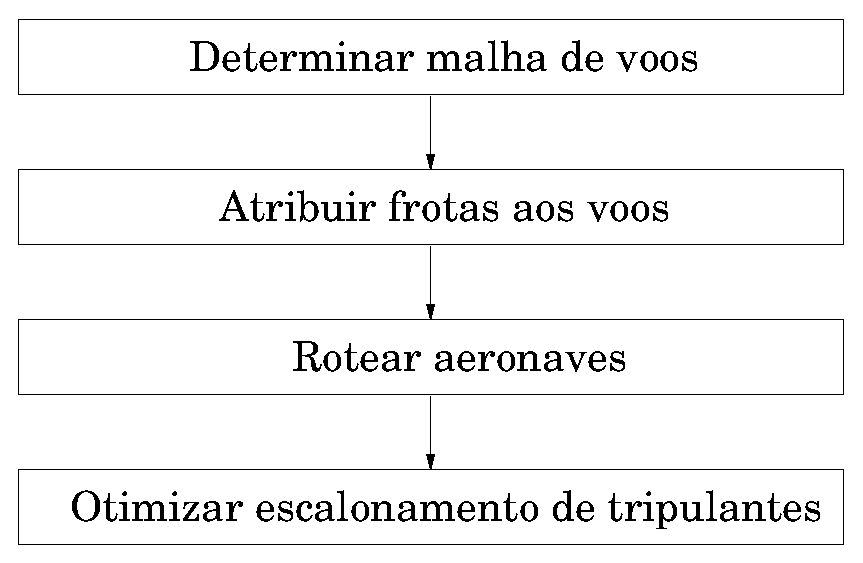
\includegraphics[scale=0.5]{fig/planejamento.eps}
		\caption{Sequência de problemas resolvidos no planejamento de operações de uma empresa
		aérea.}
		\label{fig:planejamento}
	\end{center}
\end{figure}

De forma geral, o escalonamento de tripulantes pode ser definido como o problema de se atribuir a um
grupo de trabalhadores (uma tripulação) um conjunto de atividades. No contexto da aviação, cada
tripulante (comandante, co-piloto, comissário, etc) deve ser designado para realizar um determinado
voo da empresa. Tal designação deve ser feita respeitando-se uma série de restrições impostas pelas
agências reguladoras da aviação, bem como regras de regulamentação trabalhista, restrições
operacionais impostas pela própria empresa e acordos trabalhistas entre empregado e empregador. Dado
o grande número de variáveis e restrições envolvidas, assim como a possibilidade de grandes ganhos
econômicos, o problema torna-se bastante interessante, tanto do ponto de vista da indústria, quanto
acadêmico.

Normalmente, o problema do escalonamento de tripulantes é dividido em dois subproblemas que são
resolvidos de forma independente e sequencial. O primeiro deles é conhecido como \emph{problema da
determinação de viagens} (PDV), que consiste na obtenção de um subconjunto de viagens, obedecendo as
regras de trabalho impostas pela legislação, com custo mínimo, cobrindo todas os segmentos de voo
exatamente uma vez. Obtida a solução das viagens, um segundo problema é resolvido, conhecido como
\emph{problema da determinação de escalas} (PDE), cujo objetivo é construir as escalas dos
tripulantes, distribuindo as viagens de tal forma que cada viagem seja atribuída exatamente uma vez
para cada tripulante requerido. Na atribuição, visa-se minimizar os custos e garantir distribuição
uniforme de trabalho. A atribuição das viagens também está sujeita a uma série restrições
reguladoras.

Tanto o PDV quanto o PDE têm sido extensamente estudados pela comunidade~\cite{gopalakrishnan05}. Em
especial, o primeiro deles recebeu mais atenção, principalmente no contexto norte-americano, dado o
seu potencial em produzir economia significativa de custos. No problema da determinação de escalas,
além de minimizar custos, é importante também levar em conta aspectos da qualidade de vida dos
tripulantes. Uma visão geral e esquemática dos dois problemas é apresentada na
Figura~\ref{fig:escalonamento}.

As modelagens matemáticas usuais do PDV e do PDE são semelhantes e baseiam-se em um problema de 
otimização combinatória conhecido por \emph{set partition}. A técnica de resolução comum utilizada 
pode ser descrita como ``gerar-e-otimizar''. Outras abordagens vem sendo recentemente propostas, 
buscando por soluções através de métodos meta-heurísticos. Nos próximos capítulos apresentaremos 
mais detalhes sobre as duas abordagens.

\begin{figure}[htbp]
	\begin{center}
		\includegraphics[scale=0.5]{fig/escalonamento.eps}
		\caption{Subproblemas enfrentados na solução do problema de escalonamento de tripulantes 
		(adaptado de~\cite{souai09}).}
		\label{fig:escalonamento}
	\end{center}
\end{figure}

%%%%%%%%%%%%%%%%%%%%%%%%%%%%%%%%%%%%%%%%%%%%%%%%%%%%%%%%%%%%%%%%%%%%%%%%%%%%%%%%%%%%%%%%%%%%%%%%%%%%

\section{Definições}
\label{sec:definicoes}

Antes que possamos apresentar e explorar a estrutura do problema com mais detalhes, faz-se
necessário a introdução de algumas definições e nomenclaturas usuais, as quais serão amplamente
utilizadas neste trabalho.

\begin{itemize}
	\item {\bf Etapa:} é um voo único sem paradas, também chamado de {\bf perna}, {\bf trecho} ou 
	{\bf segmento de voo}.
	\item {\bf Jornada:} conjunto de uma ou mais etapas sequenciais, também chamado de {\bf jornada 
	de trabalho}. 
	\item {\bf Tempo Mínimo de Conexão:} menor intervalo possível de tempo entre duas etapas 
	consecutivas em uma jornada.
	\item {\bf Tempo Máximo de Conexão:} maior intervalo possível de tempo entre duas etapas 
	consecutivas em uma jornada.
	\item {\bf Tempo de Briefing:} tempo mínimo que antecede o início da primeira etapa de uma
	jornada, necessário para o {\it briefing} da tripulação.
	\item {\bf Tempo de Debriefing:} tempo mínimo que sucede o término da último etapa de uma
	jornada, necessário para o {\it debriefing} da tripulação.
	\item {\bf Início da Jornada:} horário em que a tripulação deve apresentar-se para o início
	de uma jornada. Corresponde ao horário da decolagem da primeira etapa menos o tempo de 
	{\it briefing}. 
	Também chamado de {\bf checkin}.
	\item {\bf Término da Jornada:} horário em que a tripulação encerra suas atividades em uma 
	jornada. Corresponde ao horário de pouso da última etapa mais o tempo de {\it debriefing}.
	Também chamado de {\bf checkout}.
	\item {\bf Base Contratual:} cidade onde um dado tripulante está domiciliado, também
	chamada simplesmente de {\bf base}.
	\item {\bf Viagem:} conjunto de jornadas de trabalho, com a primeira etapa da primeira
	jornada e a última etapa da última jornada começando e terminando respectivamente na mesma
	base contratual. Uma viagem também é chamada de {\bf pairing}, ou {\bf rotação}.
	\item {\bf Descanso:} intervalo mínimo de tempo ininterrupto de repouso após uma jornada.
	\item {\bf Pernoite:} intervalo de tempo separando duas jornadas consecutivas de uma viagem.
\end{itemize}

A Figura~\ref{fig:viagem} apresenta o exemplo de uma viagem que ilustra alguns dos conceitos
expostos acima. As etapas na figura estão representadas pelos retângulos mais internos. São
indicados os aeroportos de origem e destino, bem como os horários de decolagem e pouso. As
jornadas são indicadas pelos retângulos pontilhados, englobando uma cadeia de etapas. A base 
contratual considerada é CGH (São Paulo). 

\begin{figure}[htbp]
	\begin{center}
		\includegraphics[scale=0.5]{fig/viagem.eps}
		\caption{Exemplo de uma viagem de dois dias para a base CGH.}
		\label{fig:viagem}
	\end{center}
\end{figure}

%%%%%%%%%%%%%%%%%%%%%%%%%%%%%%%%%%%%%%%%%%%%%%%%%%%%%%%%%%%%%%%%%%%%%%%%%%%%%%%%%%%%%%%%%%%%%%%%%%%%

\section{Formulação do PDV}
\label{sec:formulacao}

No problema da determinação das viagens, tem-se como entrada o conjunto de voos a ser operado pela
empresa, o conjunto de bases contratuais dos tripulantes, as regras de trabalho que ditam a
construção de viagens legais e uma estrutura de custo (mais detalhes na 
Seção~\ref{sec:regras_e_custos}). A saída, então, deve ser um conjunto de viagens que cubra todos os
voos operados exatamente e uma vez e que tenha o custo mínimo (veja Figura~\ref{fig:pdv}).

\begin{figure}[htbp]
	\begin{center}
		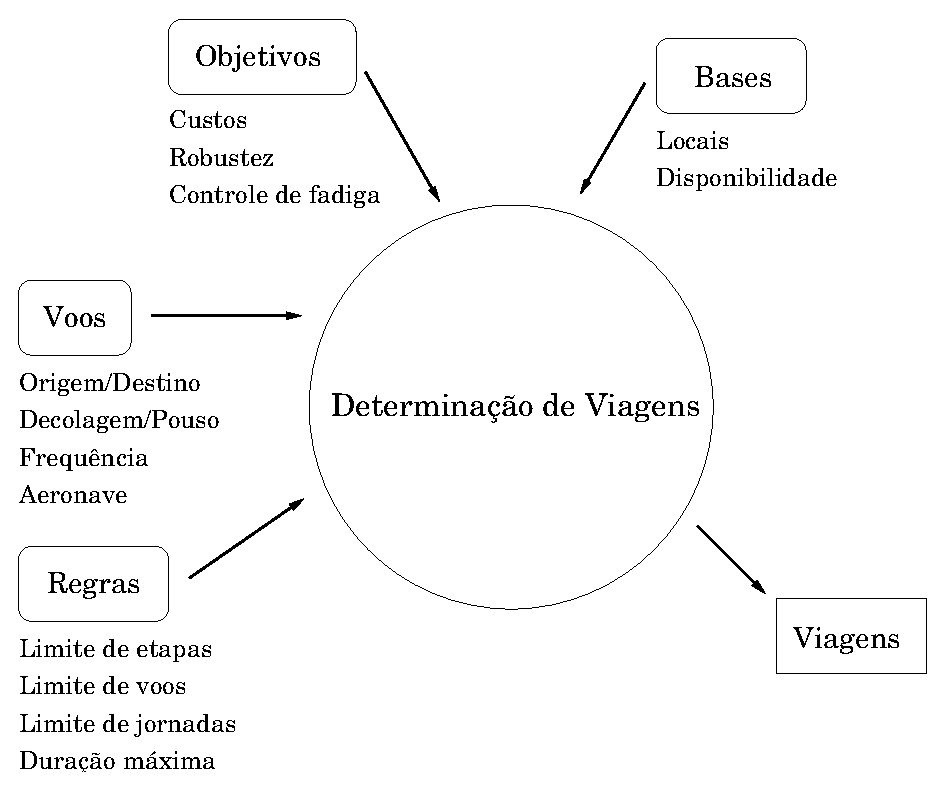
\includegraphics[scale=0.5]{fig/pdv.eps}
		\caption{Representação do problema da determinação de viagens (PDV).}
		\label{fig:pdv}
	\end{center}
\end{figure}

Normalmente os voos das companhias aéreas apresentam uma frequência regular de oferecimento, sendo
que a maioria deles operam diariamente. Outros são oferecidos apenas em alguns dias fixos da semana
e poucos são oferecidos vez ou outra no mês. Costuma-se então inicialmente resolver o problema
diário, onde se assume que todos os voos são repetidos diariamente. Note que, para o problema
diário, viagens de vários dias com etapas repetidas são inviáveis. Um segmento de voo repetido
causaria o efeito de mais de uma tripulação ser atribuída para realização dessa etapa, uma vez que
quando se faz a implementação da solução diária, uma tripulação distinta é atribuída a cada um dos
dias da viagem.

O problema semanal é mais complicado porque envolve um maior número de etapas consideradas. De
qualquer forma, a solução do problema semanal pode ser obtida a partir de um ajuste da solução do
problema diário, sem perda significativa de custo~\cite{gopalakrishnan05}. A solução do problema
mensal completo segue da solução do problema semanal. Como a maior parte da redução de custos está
associada à resolução do problema diário, ele torna-se o mais importante. Daqui em diante trataremos
apenas do problema diário.

Uma outra simplificação do problema está no fato de que os tripulantes são habilitados para operar
apenas um tipo, ou família, de aeronaves dentro de uma frota. Assim, fatora-se o problema da
determinação das viagens por tipo de aeronave. Para cada tipo, resolve-se um PDV considerando apenas
as etapas operadas por ele. No PDE, as viagens assim geradas são atribuídas apenas a tripulantes
habilitados a operar cada tipo de aeronave.

Há uma formulação natural para o PDV em termos de um problema de programação linear. Suponha que
seja possível gerar e enumerar todas as $n$ viagens associadas a uma dada entrada do problema
contendo $m$ etapas a serem cobertas. Seja $x_j \in \{0, 1\}$ uma variável de decisão que assume o
valor 1 se a viagem $j$ for escolhida na solução de custo mínimo e 0 caso contrário. Então, o PDV
pode ser modelado da seguinte forma:
%
\begin{eqnarray} \label{eq:sppv}
	\text{minimizar} && \displaystyle \sum_{j=1}^n c_j x_j \nonumber \\
	\text{sujeito à} && \displaystyle \sum_{j=1}^n a_{ij} x_j = 1 \ev \;\; i = 1, \ldots, m \\
		               && x_j \in \{0, 1\} \ev \;\; j = 1, \ldots, n \ep \nonumber
\end{eqnarray} 
%
Os coeficientes $a_{ij}$ são definidos por (matriz de incidência)
%
\begin{equation*}
	a_{ij} = \left\{
	\begin{array}{ll}
			1 \ev & \text{se a viagem $j$ cobre a etapa $i$} \\
			0 \ev & \text{caso contrário}
	\end{array}
	\right.
\end{equation*}

As restrições em (\ref{eq:sppv}) garantem que cada etapa seja coberta exatamente uma vez por alguma
viagem. Existe ainda uma formulação alternativa onde as restrições são dadas por
%
\begin{equation} \label{eq:dh} 
	\sum_{j=1}^n a_{ij} x_j \geq 1 \, , \;\; i = 1, \ldots, m \ep
\end{equation} 
%
Nesse caso uma mesma etapa pode ser coberta por mais de uma viagem e o problema passa a ser
denominado \emph{set cover}. Do ponto de vista do escalonamento, se uma etapa é coberta por mais
de uma viagem, então uma tripulação estará trabalhando nessa etapa e as demais viajando de
passageiro (situação conhecida por \emph{deadheading}). Às vezes, essa situação é necessária para
que se garanta a viabilidade da solução. Se o preço a se pagar pela operação com \emph{deadheading} 
for essencialmente o mesmo de uma operação normal, então não há alteração significativa no custo 
da viagem associada. Isso permite que o problema seja modelado com as restrições (\ref{eq:dh}) 
sem alterar a estrutura de custos.

É comum a inserção de restrições adicionais ao modelo que garantem uma distribuição de trabalho
entre as bases compatível com os recursos disponíveis em cada uma. Se o número total de bases do
problema considerado é $r$, então as \emph{restrições de bases} são expressas por
%
\begin{equation} \label{eq:bases}
	H_k^L \leq \sum_{j=1}^n h_{kj} x_j \leq H_k^U \, , \;\; k = 1, \ldots, r \ev
\end{equation}
%
onde $H_k^L$ é o número mínimo de horas disponíveis na base $k$ e $H_k^U$ é seu número máximo. 
Note que $H_k^L$ pode ser diferente de zero desde que se exija que não mais do que um certo número 
de tripulantes fique de reserva. O coeficiente $h_{kj}$ dá o número de horas necessárias para 
efetuar a viagem $j$ ($h_{kj} = 0$ se a viagem $j$ não pertencer à base $k$).

O grande problema com a formulação (\ref{eq:sppv}) está no enorme número de variáveis geradas, mesmo
nos casos das instâncias pequenas (poucas etapas diárias). A Tabela~\ref{tab:viagens} ilustra o
número de viagens legais geradas, com duração máxima de 3 ou 4 dias, para diversas frotas de
aeronaves. O número enorme de variáveis está associada com a natureza combinatória do problema. A
maioria das empresas aéreas operam em aeroportos conhecidos como \emph{hubs}, onde um grande número
de aeronaves chegam e partem em um mesmo intervalo de tempo, possibilitando que os passageiros
efetuem suas conexões para uma variedade de destinos em pouco tempo. Esse tipo de estrutura em rede 
leva à explosão no número de viagens legais que podem ser construídas~\cite{graves93}. Note na
Tabela~\ref{tab:viagens} que, apesar do número de viagens ser gigantesco, o número de 
jornadas tem um valor mais gerenciável.

\begin{table}[ht]
	\begin{center}
		\begin{tabular}{|c||c|c|c|c|c|}
			\hline
			{\bf Frota} & {\bf Max Dias} & {\bf Etapas} & {\bf Bases} & {\bf Jornadas} & 
			{\bf Viagens} ($\times 10^6$) \\
			\hline
			AAS80 & 3 & 1.152 & 12 & 690.000 & 48.400 \\
			\hline
			AA757 & 3 & 251 & 15 & 7.000 & 1 \\
			\hline
			AA727 & 3 & 375 & 11 & 31.000 & 36 \\
			\hline
			AAF10 & 4 & 307 & 3 & 55.000 & 63.200 \\
			\hline 
			UA737 & 4 & 773 & 7 & 568.000 & 100.000.000 \\
			\hline
			USDC9 & 4 & 478 & 4 & 562.000 & 105.000.000 \\
			\hline
		\end{tabular}
		\caption{Jornadas e viagens legais geradas para um conjunto de frotas de aeronaves de companhias
		norte-americanas (fonte:~\cite{anbil98}).}
		\label{tab:viagens}
	\end{center}
\end{table}

Como o problema de partição é NP-difícil~\cite{garey79}, a aplicação de métodos diretos de
otimização é impraticável para qualquer situação real. Discutiremos esse ponto na
Seção~\ref{sec:preliminar}. Os métodos de solução normalmente envolvem algum tipo de heurística e/ou
algum critério de parada que leva a soluções sub-ótimas.

%%%%%%%%%%%%%%%%%%%%%%%%%%%%%%%%%%%%%%%%%%%%%%%%%%%%%%%%%%%%%%%%%%%%%%%%%%%%%%%%%%%%%%%%%%%%%%%%%%%%

\section{Objetivos e Estrutura}
\label{sec:objetivos}

Neste trabalho focamos no problema da determinação das viagens. Os objetivos foram estudar a 
literatura, entender e implementar alguns dos métodos de solução disponíveis, aplicando-os
no contexto de companhias aéreas brasileiras e, por fim, analisar os resultados obtidos.

O contexto brasileiro difere significativamente dos contextos estrangeiros no que refere-se à 
estrutura de custos e regras que ditam a viabilidade de uma viagem. Como os trabalhos estudados na
literatura referem-se ao escopo norte-americano e europeu, tivemos por objetivo também efetuar as 
devidas adaptações na tentativa de solucionar problemas de companhias aéreas brasileiras.

Esta monografia está estruturada da seguinte forma: neste capítulo faz-se uma introdução e
contextualização do problema em estudo. Em seguida, no Capítulo~\ref{cap:geracao}, apresentamos o
método de geração de viagens, com destaque especial na estrutura de custos e regras de viabilidade,
e um exemplo explícito é apresentado. No Capítulo~\ref{cap:heuristicas}, apresentamos as três
heurísticas implementadas neste trabalho, a saber, um método de busca local, um algoritmo genético
híbrido e um procedimento de geração de colunas. O Capítulo~\ref{cap:resultados} mostra os
resultados obtidos aplicando-se as heurísticas estudadas a algumas instâncias reais do problema. Em
particular, mostramos a redução do custo da solução em função do número de iterações que controla a
evolução dos algoritmos. Finalmente, no Capítulo~\ref{cap:conclusao}, destacamos algumas conclusões
e comparações de resultados. Listamos também alguns pontos de melhorias, dificuldades com o projeto
e perspectivas futuras.

A segunda parte desta monografia apresenta o conteúdo subjetivo, destacando a opinião e as
impressões de cada autor sobre o curso do BCC/IME e sua relação com este projeto
(Capítulo~\ref{cap:analise_subjetiva}).

\zerar
\chapter{Geração de Viagens}
\label{cap:geracao}

Todos os métodos de solução do PDV (exatos ou heurísticos) exigem um mecanismo de geração 
explícita de viagens legais, as quais representam as variáveis que desejamos otimizar. 

A geração pode ser eficientemente implementada através de uma busca em uma rede de voos. 
O resultado da busca depende explicitamente das regras de trabalho impostas pelo contexto do
problema. As viagens geradas apresentam um custo também intimamente ligado ao contexto e ao 
objetivo que se deseja atingir. 

Neste capítulo apresentaremos mais detalhes sobre o procedimento de geração de viagens. Ao final,
será exibido um exemplo explícito.

%%%%%%%%%%%%%%%%%%%%%%%%%%%%%%%%%%%%%%%%%%%%%%%%%%%%%%%%%%%%%%%%%%%%%%%%%%%%%%%%%%%%%%%%%%%%%%%%%%%%

\section{Regras de Trabalho e Estrutura de Custo}
\label{sec:regras_e_custos}

É importante explicitar os tipos de restrições e a estrutura de custo envolvidos no problema, em 
especial no contexto brasileiro, já que há uma diferença significativa com relação aos contextos 
norte-americano e europeu, normalmente analisados na literatura.

No caso do PDV, a geração de uma viagem é regida por uma série de regras impostas pela Agência
Nacional de Aviação Civil (ANAC), além de restrições impostas por leis trabalhistas e acordos
contratuais. Uma viagem é dita legal se ela obedecer todas as regras impostas pela legislação em
questão. Abaixo, apresentamos os valores típicos das regras que regem a construção de uma viagem
em uma empresa de aviação regular do Brasil, com voos de curto e médio alcance (veja a
Seção~\ref{sec:definicoes} para as defininições):

\begin{itemize}
	\item Duração máxima de uma jornada de trabalho: 11 horas;
	\item Número máximo de horas de voo em uma jornada: 9 horas e 30 minutos;
	\item Número máximo de pousos em uma jornada: 6 pousos;
	\item Descanso mínimo entre jornadas: 12 horas;
	\item Tamanho máximo de uma viagem: 6 dias;
	\item Tempo mínimo de conexão: 30 minutos;
	\item Tempo máximo de conexão: 4 horas;
	\item Número máximo de trocas de aeronave em uma jornada: 2 trocas;
	\item Tempo de {\it briefing}: 30 minutos fora de base e 45 minutos na base;
	\item Tempo de {\it debriefing}: 30 minutos.
\end{itemize}

O custo de uma viagem está associado à produtividade mais os custos referentes à estadia do 
tripulante quando este precisar pernoitar fora da base, além das diárias de alimentação. Uma 
expressão típica para calcular o custo $c_p$ de uma viagem $p$ é dada por
%
\begin{equation} \label{eq:custov} 
	c_p = \sum_{d \in D_p} c_d \, , \;\;
	c_d = \alpha_0 \left[t_d - \left(tp_d - \sum_{i \in I_d} t_i\right)\right] + cp_d \ev
\end{equation} 
%
onde
%
\begin{itemize}
	\item[$D_p$:] conjunto de jornadas que constituem a viagem $p$;
	\item[$c_d$:] custo da jornada $d$;
	\item[$\alpha_0$:] custo da hora de trabalho do tripulante;
	\item[$t_d$:] duração da jornada $d$ (em horas);	
	\item[$tp_d$:] tempo de preparação ({\it briefing} mais {\it debriefing}) usado na jornada $d$;
	\item[$I_d$:] conjunto de etapas que compõe a jornada $d$;
	\item[$t_i$:] duração da etapa $i$, incluindo o tempo mínimo de conexão;
	\item[$cp_d$:] custo do pernoite mais diárias de alimentação da jornada $d$.
\end{itemize}
%
Note que a expressão que multiplica $\alpha_0$ em (\ref{eq:custov}) representa o tempo que o
tripulante passou trabalhando sem estar voando, portanto representa uma medida de produtividade.
Quanto mais cara a viagem, menor é a produtividade do tripulante.

A estrutura descrita acima refere-se a um modelo padrão para companhias aéreas brasileiras.
Fora do Brasil, entretanto, a estrutura do custos pode ser diferente. Nos Estados Unidos, por 
exemplo, o custo de uma viagem é dado por uma função não-linear de diferentes custos. 
Especificamente, o custo de uma viagem $p$ é dado por
%
\begin{equation*}
	c_p = \max\left\{\sum_{d \in D_p} MIN\_GRT_d \ev \sum_{d \in D_p} FLY\_TIME_d \ev 
	TIME\_AWAY_p \right\} \ev
\end{equation*}
%
onde $MIN\_GRT_d$ é o mínimo de garantia oferecido ao tripulante ao voar a jornada $d$, 
$FLY\_TIME_d$ é o tempo de voo da jornada $d$ (pode ser multiplicado por algum fator) e
$TIME\_AWAY_p$ é o tempo total que o tripulante passa fora de sua base na viagem $p$ (também pode
ser multiplicado por algum fator). Observe assim que, nesse modelo, o custo de cada etapa depende da
viagem em ela está incluída.

%%%%%%%%%%%%%%%%%%%%%%%%%%%%%%%%%%%%%%%%%%%%%%%%%%%%%%%%%%%%%%%%%%%%%%%%%%%%%%%%%%%%%%%%%%%%%%%%%%%%

\section{Gerador de Viagens}
\label{sec:gerador_viagens}

O primeiro passo em direção à solução do PDV consiste na implementação de um gerador de viagens 
eficiente que seja capaz de produzir um grande número de viagens legais em pouco tempo. Como já
mencionamos, os métodos de resolução de (\ref{eq:sppv}) baseiam-se no conceito de 
``gerar-e-otimizar'', e já que as rotinas de otimização estão normalmente prontas em pacotes 
fechados, a parte de geração é de grande importância.

Uma viagem pode ser vista como um caminho especial em um grafo estruturado. Esse grafo é chamado de
\emph{rede de voos} e será detalhado a seguir. 

As etapas na rede de voos podem ser representadas como nós ou arcos. Escolhemos a representação em
termos de arcos. Os nós da rede representam as saídas e chegadas de cada etapa, bem como uma fonte
$s$ e um sorvedouro $t$. Existe um arco representando cada etapa da malha de voos. Para o problema
diário, replicamos cada arco quantas vezes for o número máximo de dias permitido em um viagem. O
conjunto de arcos será denotado por $\calA$.

O nó fonte é ligado ao nó de saída de cada etapa que origina-se em uma base específica. O nó de
chegada de cada etapa que termina nessa base é ligado ao sorvedouro. Existem ainda arcos
representando conexões legais entre etapas. Um par de etapas terá um arco de conexão entre elas se
o aeroporto de chegada do primeiro corresponder ao aeroporto de saída do segundo e se o intervalo de
tempo entre a chegada e a saída estiver dentro dos limites necessários para se estabelecer uma
conexão legal em uma jornada ou descanso regular entre jornadas. 

É fácil notar que toda viagem legal é representada por um caminho $s-t$ na rede de voos. Porém,
existem caminhos $s-t$ que não representam viagens legais pois podem desrespeitar alguma regra de
trabalho, embora as conexões possíveis sejam legais. A estrutura da rede garante que não seja feita
nenhuma conexão entre duas etapas que não tenham seus respectivos destino e origem coincidentes no
espaço e no tempo. Entretanto, não garante, por exemplo, que o número máximo de horas de voo
permitido em uma jornada seja excedido. 

O gerador de viagens funciona aplicando um algoritmo de busca em profundidade à rede de voos. O
algoritmo inicia-se no nó de origem $s$ e explora todas a conexões viáveis $(i, j) \in \calA$, até
retroceder. O processo de busca em profundidade controla a viabilidade das viagens, levando em conta
a duração máxima das jornadas, limites de horas de voo e de pousos, etc (ou seja, verifica as regras
de trabalho ao atravessar cada arco).

%%%%%%%%%%%%%%%%%%%%%%%%%%%%%%%%%%%%%%%%%%%%%%%%%%%%%%%%%%%%%%%%%%%%%%%%%%%%%%%%%%%%%%%%%%%%%%%%%%%%

\section{Exemplo}
\label{sec:exemplo}

A tabela abaixo mostra um conjunto fictício (para fins de ilustração) de 7 etapas operadas 
diariamente entre as localidades A, B, C e D. O exemplo é adaptado de~\cite{barnhart03}. 

\begin{table}[ht]
	\begin{center}
		\begin{tabular}{ccccc}
			{\bf \# Etapa} & {\bf Origem} & {\bf Destino} & {\bf Saída} & {\bf Chegada} \\ \hline
			1 & A & B & 08:00 & 09:00 \\
			2 & B & C & 10:00 & 11:00 \\
			3 & C & D & 13:00 & 14:00 \\
			4 & C & A & 15:00 & 16:00 \\
			5 & D & A & 15:00 & 16:00 \\
			6 & A & B & 17:00 & 18:00 \\
			7 & B & C & 11:00 & 12:00 \\
		\end{tabular}
	\end{center}
\end{table}

A rede de voos (parcial) para uma base contratual A é ilustrada na Figura~\ref{fig:rede}, onde são
apresentadas algumas das conexões legais possíveis para clareza do desenho. O caminho vermelho
na figura representa uma viagem legal com dois dias de duração. 

A partir da rede apresentada, montamos as seguintes jornadas válidas (os números representam os
números das etapas)
%
\begin{eqnarray*}
	&& D_1 = \{1\} \ev \hsp D_2 = \{2\} \ev \hsp D_3 = \{3\} \ev \hsp D_4 = \{4\} \\
	&& D_5 = \{5\} \ev \hsp D_6 = \{6\} \ev \hsp D_7 = \{7\} \ev \hsp D_8 = \{1, 2\} \\
	&& D_9 = \{1, 7 ,3\} \ev \hsp D_{10} = \{2, 3\} \ep 
\end{eqnarray*}

Assumindo que as localidades A, B e D sejam bases contratuais, geramos seis viagens, que podem ser
expressas em termos das jornadas como 
%
\begin{eqnarray*}
	&& P_1 = \{D_4, D_8\} \ev \hsp P_2 = \{D_9, D_5\} \ev \hsp P_3 = \{D_5, D_6, D_{10}\} \\
	&& P_4 = \{D_4, D_6, D_7\} \ev \hsp P_5 = \{D_1, D_7, D_4\} \ev \hsp P_6 = \{D_7, D_4, D_9\}
\ep 
\end{eqnarray*}

Note que a viagem $P_6$ cobre a etapa $7$ duas vezes, então ela não é válida e deve ser 
desconsiderada. Supondo que os custos associados às viagens sejam $c_1 = c_2 = c_3 = c_4 = 4$ e
$c_5 = 5$, a partir de (\ref{eq:sppv}) obtemos o seguinte problema ($x_i \in \{0, 1\}$, 
$i=1, \ldots, 5$):
%
\begin{equation*}
	\begin{array}{lllllllllllll}
		\text{min} & 4x_1 & + & 4x_2 & + & 4x_3 & + & 4x_4 & + & 5 x_5 & & & \vsp \\ 
		& x_1 & + & x_2 & & & & & + & x_5 & = & 1 & \text{(etapa 1)} \vsp \\
		& x_1 & & & + & x_3 & & & & & = & 1 & \text{(etapa 2)} \vsp \\
		& & & x_2 & + & x_3 & & & & & = & 1 & \text{(etapa 3)} \vsp \\
		& x_1 & & & & & + & x_4 & + & x_5 & = & 1 & \text{(etapa 4)} \vsp \\
		& & & x_2 & + & x_3 & & & & & = & 1 & \text{(etapa 5)} \vsp \\
		& & & & & x_3 & + & x_4 & & & = & 1 & \text{(etapa 6)} \vsp \\
		& & & x_2 & & & + & x_4 & + & x_5 & = & 1 & \text{(etapa 7)}
	\end{array}
\end{equation*}

Se pelo menos 3 horas e no máximo 6 horas estejam disponíveis nas bases A e D, e no máximo 5 horas 
na base C, então as restrições de bases (\ref{eq:bases}) são
%
\begin{equation*}
	\begin{array}{ll}
		3 \leq 4 x_2 + 3 x_5 \leq 6 & \text{(base A)} \vsp \\
		0 \leq 3 x_1 + 3 x_4 \leq 5 & \text{(base C)} \vsp \\
		3 \leq 4 x_3 \leq 6 & \text{(base D)}
	\end{array}
\end{equation*}

A solução ótima para o problema formulado usa as viagens 3 e 5 ($x_3 = x_5 = 1$, 
$x_1 = x_2 = x_4 =  0$) e tem um custo total igual à 9. Por se tratar de um problema pequeno, a
resolução do mesmo pode ser obtida por qualquer pacote de otimização linear.

\begin{figure}[htbp]
	\begin{center}
		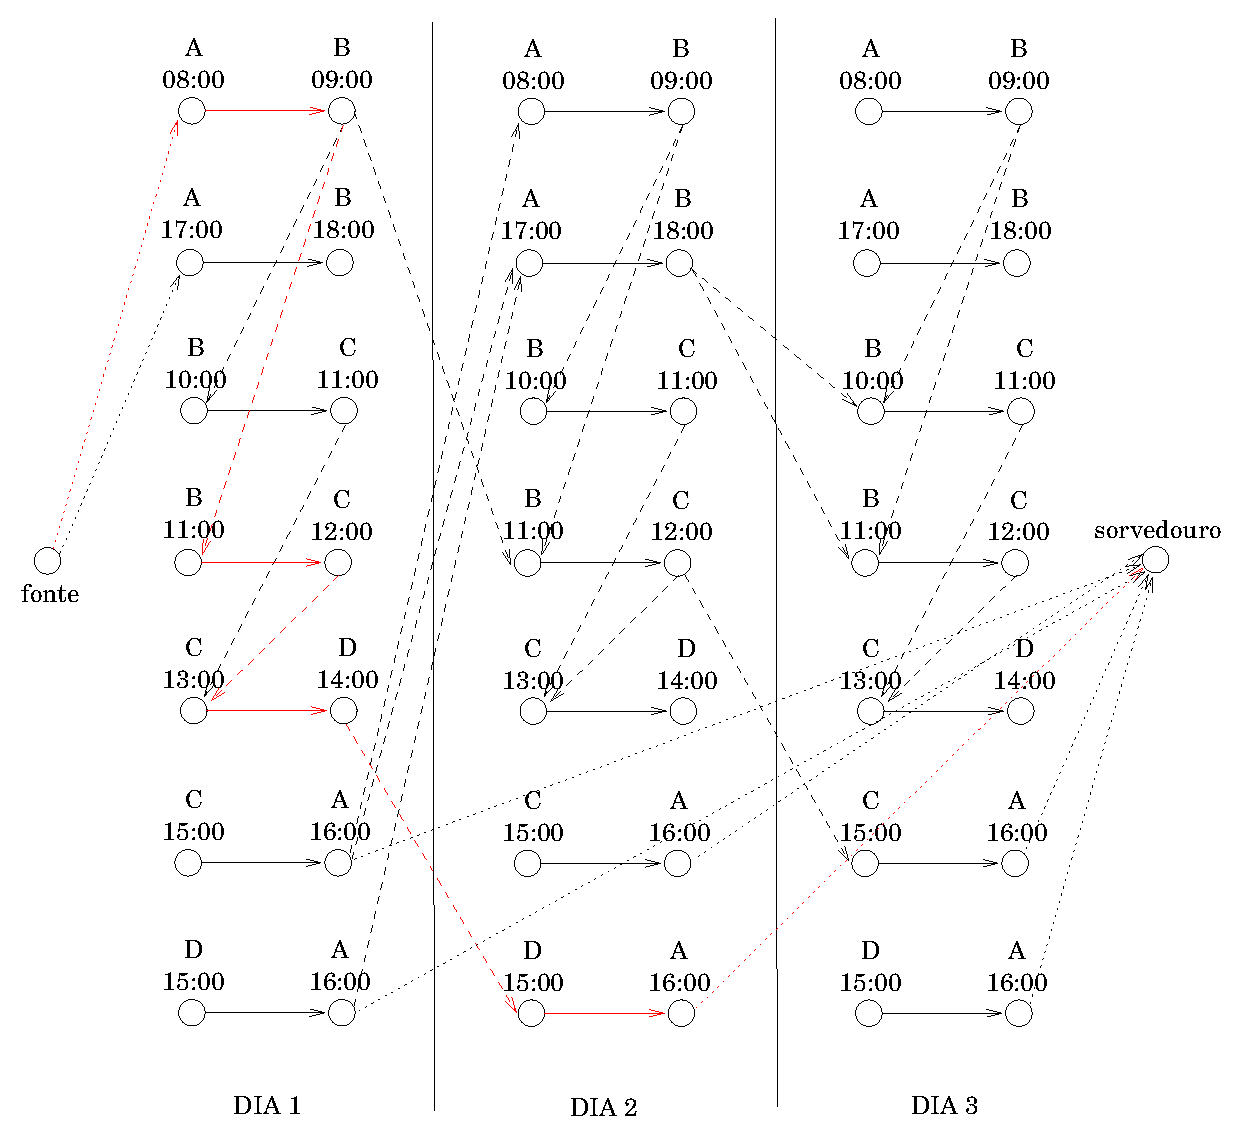
\includegraphics[scale=0.80]{fig/rede.eps}
		\caption{Rede de voos referente às 7 etapas do exemplo ilustrativo. Considerou-se
		viagens de no máximo 3 dias, por isso os nós são replicados três vezes para o
		problema diário. A base dos tripulantes considerada foi a localidade A, dando origem
		às ligações da fonte e do sorvedouro.
		Arcos tracejados representam conexões legais entre localidades. O caminho em vermelho representa
		uma das viagens possíveis.}
		\label{fig:rede}
	\end{center}
\end{figure}

%%%%%%%%%%%%%%%%%%%%%%%%%%%%%%%%%%%%%%%%%%%%%%%%%%%%%%%%%%%%%%%%%%%%%%%%%%%%%%%%%%%%%%%%%%%%%%%%%%%%


\zerar
\chapter{Heurísticas}
\label{cap:heuristicas}


%%%%%%%%%%%%%%%%%%%%%%%%%%%%%%%%%%%%%%%%%%%%%%%%%%%%%%%%%%%%%%%%%%%%%%%%%%%%%%%%%%%%%%%%%%%%%%%%%%%%

\section{Busca Local}
\label{sec:metodos_busca}

O método de busca local é bastante simples e foi um dos primeiros a ser utilizado na tentativa de 
melhorar uma solução viável do problema (\ref{eq:scpdv}). 

A busca local consiste em escolher aleatoriamente duas ou três viagens da solução viável inicial e, 
a partir da lista de etapas cobertas por essas viagens, gerar explicitamente todas as possíveis 
viagens legais usando o gerador. Como o número de etapas não é muito grande, o número de variáveis 
geradas é gerenciável. O modelo (\ref{eq:scpdv}) é então resolvido para todas essas variáveis, 
obtendo um novo conjunto de viagens que cobre o lista de etapas inicial. 

Se o custo desse novo conjunto de viagens for menor do que o original, então as viagens originais
serão substituídas na solução global. O processo é iterado um número máximo de vezes (ou um tempo 
máximo de execução), ou até que não haja variação significativa do custo (mínimo local), de tal 
forma que o custo sempre seja reduzido a cada passo.

%%%%%%%%%%%%%%%%%%%%%%%%%%%%%%%%%%%%%%%%%%%%%%%%%%%%%%%%%%%%%%%%%%%%%%%%%%%%%%%%%%%%%%%%%%%%%%%%%%%%

\section{Algoritmo Genético}
\label{sec:metodos_genetico}

Daremos aqui a formulação de um algoritmo genético para o problema (\ref{eq:scpdv}). 

%%%%%%%%%%%%%%%%%%%%%%%%%%%%%%%%%%%%%%%%%%%%%%%%%%%%%%%%%%%%%%%%%%%%%%%%%%%%%%%%%%%%%%%%%%%%%%%%%%%%

\section{Geração de Colunas}
\label{sec:metodos_colunas}

Nesta seção descreveremos o método de geração de colunas para obtenção de uma solução ótima 
associada ao problema em (\ref{eq:scpdv}), chamado de problema mestre.

A ideia básica consiste em não gerar explicitamente todas as $n$ viagens possíveis do problema. 
Ao invés disso, começamos com um número reduzido de colunas que forneça ao menos uma solução viável
(o chamado problema restrito). Essas variáveis são levadas ao otimizador considerando a versão 
relaxada de (\ref{eq:scpdv}). Para determinar se o problema original com todas as $n$ variáveis 
está resolvido otimamente, solucionamos o seguinte subproblema:
%
\begin{equation} \label{eq:sub}
	w^\ast = \min_{j = 1, \ldots, n} \left[ c_j - \sum_{i=1}^m \pi_i a_{ij} \right] \ev
\end{equation} 
%
onde $\pi_i$, $i = 1, \ldots, m$ são as variáveis duais ótimas associadas ao problema restrito.
Da teoria da programação linear, sabemos que se $w^\ast \geq 0$ então o problema restrito é ótimo
ao problema mestre. Por outro lado, se  $w^\ast < 0$, a coluna $k$ (com custo reduzido 
$\bar{c}_k < 0$) é identificada e é adicionada ao problema restrito. O problema restrito é 
resolvido novamente e o processo se repete até que nenhuma variável de custo reduzido negativo 
seja encontrada.

Ocorre que o subproblema (\ref{eq:sub}) pode ser traduzido como um problema de caminho mais curto 
no grafo da rede de voos, o qual pode ser resolvido de forma eficiente. Mostraremos isso com mais 
detalhes na próxima versão deste trabalho.



\zerar
\chapter{Resultados}
\label{cap:resultados}

Em nosso estudo, utilizamos os pacotes de otimização GLPK (GNU Linear Programming Kit) e Cplex da
IBM. Os resultados finais, entretanto, são baseados apenas na utilização da ferramenta Cplex, uma
vez que a mesma provou ser mais eficiente. Além disso, o otimizador Cplex pôde ser utilizado
diretamente a partir de nosso código, alimentando o modelo gerado através da API Java fornecida pela
IBM. Por outro lado, como o GLPK não fornece API apropriada, sua utilização se limitou a geração do
modelo em arquivo (formato mps) e posterior execução do otimizador em um processo separado, sendo
necessário realizer um {\it parsing} no arquivo de saída gerado para obtenção dos resultados.

Restringimos o nosso estudo de escalonamento à resolução do problema de determinação de viagens.
Implementamos os métodos de solução do PDV descritos na Seção~\ref{sec:metodos}. Os parâmetros 
utilizados, que garantem a legalidade das viagens geradas, são apresentados na 
Tabela~\ref{tab:parametros} e baseiam-se na legislação brasileira para aviação comercial regular. 

Todos os testes foram realizados em um computador utilizando um processador Intel Core~i3 64~bits, 
com 4~Gb de memória RAM, rodando o sistema operacional MacOS~10.6. Toda a implementação foi escrita 
em Java (JDK~1.6.33).

\begin{table}
	\begin{center}
		\begin{tabular}{|l|l|l|}
			\hline 
			\bf Parâmetro & \bf Descrição & \bf Valor \\
			\hline \hline 
			\verb|MAX_LEGS| & Máximo de pernas por jornada & 5 \\ \hline
			\verb|MAX_FLIGHT_TIME| & Total máximo de voo por jornada & 9,5 h \\ \hline
			\verb|MAX_DUTY_TIME| & Duração máxima de uma jornada & 11,5 h \\ \hline
			\verb|MIN_SIT_TIME| & Tempo mínimo de conexão & 30 min \\ \hline
			\verb|MAX_SIT_TIME| & Tempo máximo de conexão & 120 min \\ \hline
			\verb|BRIEFING_TIME| & Tempo para o {\it briefing} & 0 min \\ \hline
			\verb|DEBRIEFING_TIME| & Tempo para o {\it debriefing} & 0 min \\ \hline
			\verb|MIN_REST_TIME| & Tempo mínimo de repouso & 12 h \\ \hline
			\verb|MAX_REST_TIME| & Tempo máximo de repouso & 36 h \\ \hline
			\verb|MAX_DUTIES| & Máximo de jornadas por viagem & 2, 3 ou 4 \\ \hline
			\end{tabular} 
			\caption{Parâmetros utilizados na geração das viagens.}
			\label{tab:parametros}
	\end{center}
\end{table}

%%%%%%%%%%%%%%%%%%%%%%%%%%%%%%%%%%%%%%%%%%%%%%%%%%%%%%%%%%%%%%%%%%%%%%%%%%%%%%%%%%%%%%%%%%%%%%%%%%%%

\section{Análise Preliminar}
\label{sec:analise_p}

O objetivo desta análise preliminar foi definir o limite de utilização do procedimento de geração
de viagens e do otimizador na resolução exata do modelo {\it set partition} (\ref{eq:sppv}).
Com essa finalidade, construímos alguns gráficos que relacionam o tempo de geração e otimiazação 
utilizado em nossa implementação, em função do número de etapas dadas como entrada do problema.

Para estudar a influência do número de pernas isoladamente, restringimos a entrada apenas para um
conjunto de voos entre duas localidades, São Paulo (CGH) e Rio de Janeiro (SDU), considerando os
trechos diárias oferecidos na ponte-aérea pela companhia aérea Gol. Um total de 62 pernas 
(31 de CGH para SDU e 31 de SDU para CGH) representam a instância global de entrada.

Vale observar que o caso da ponte-aérea é um pouco atípico no sentido de que representa um malha 
muito densa de voos: muitas etapas são oferecidas de ida e volta num curto intervalo de tempo, 
criando muitas conexões legais (arcos) entre os nós da rede de voos gerada. Com isso, o número
de viagens dado pela procedimento de busca no grafo explode rapidamente.

O gráfico da Figura~\ref{fig:pairings} mostra o número de viagens geradas em função do número de
etapas na ponte-aérea. As viagens foram geradas para a base CGH. São apresentadas três curvas, uma
para cada valor do parâmetro \verb|MAX_DUTIES| (2, 3 e 4). Observe a escala logarítmica do eixo
vertical. O comportamento praticamente linear das curvas indica um crescimento exponencial do número
de viagens que podem ser geradas. Observe ainda que a taxa de crescimento é maior quanto maior o
número máximo de jornadas permitidas, já que nesse caso permite-se um número muito maior de
combinações. Para \verb|MAX_DUTIES| = 4, encontrou-se um número da ordem de $10^8$ viagens com
apenas 36 pernas.

\begin{figure}[htp]
	\begin{center}
		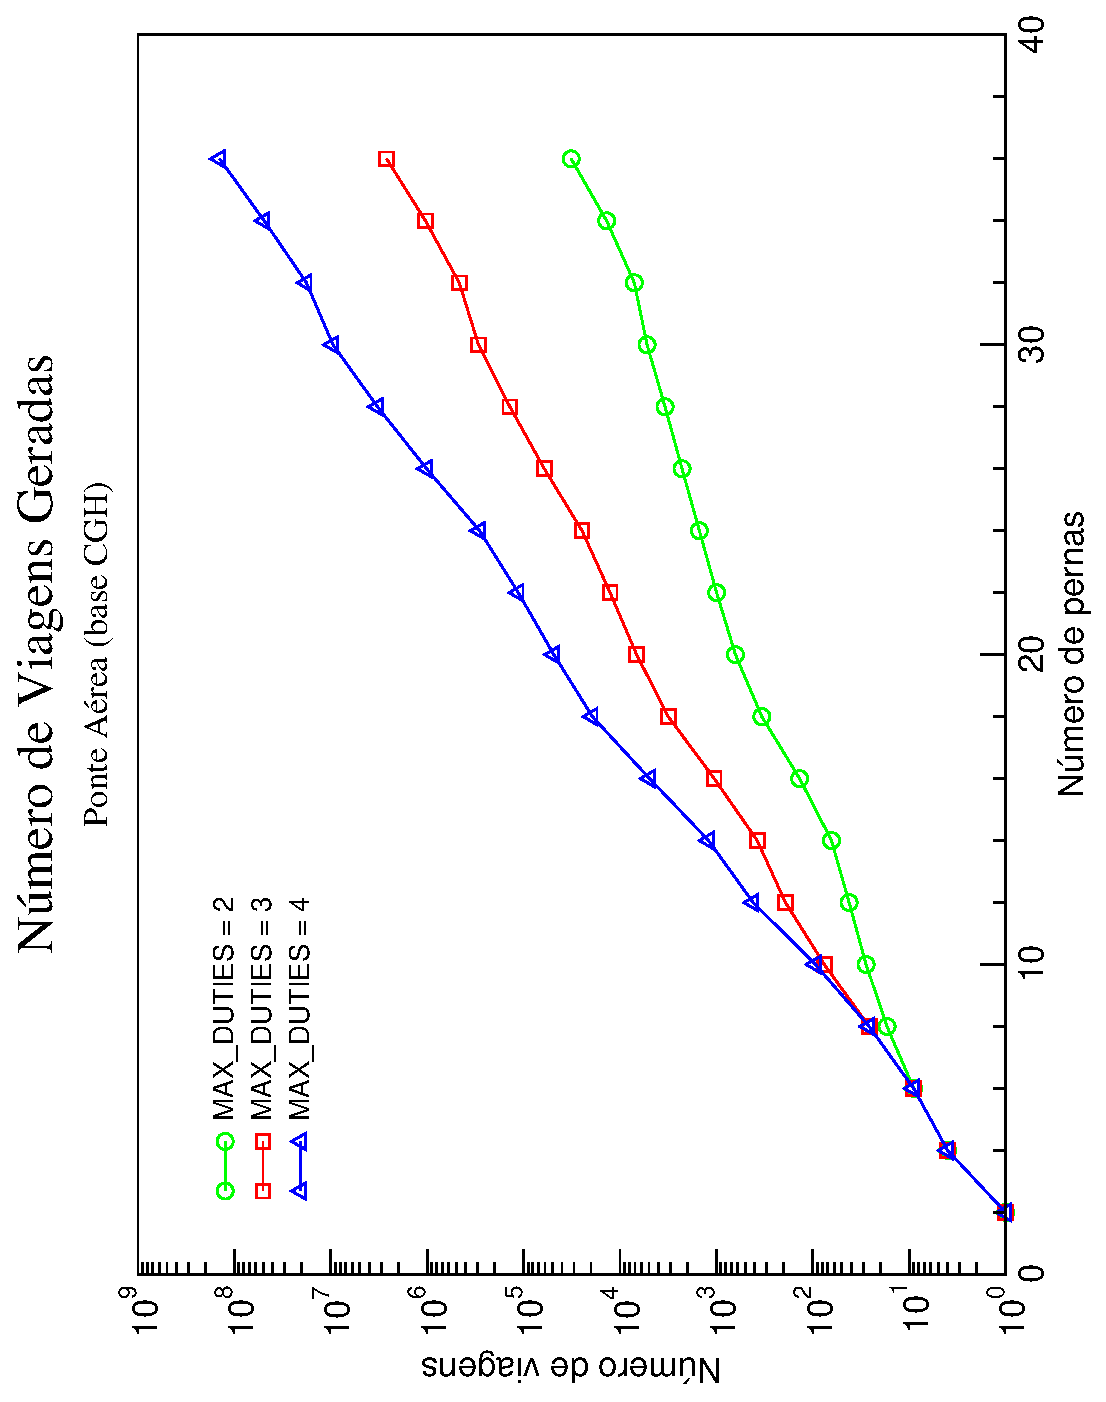
\includegraphics[scale=0.45,angle=-90]{fig/number_of_pairings.eps}
		\caption{Número de viagens geradas em função do número de pernas utilizadas na construção da
		rede de voos.}
		\label{fig:pairings}
	\end{center}
\end{figure}

O consumo de tempo gasto pelo algoritmo de busca em profundidade também foi medido em função do 
número de pernas. Os resultados são apresentados na Figura~\ref{fig:generation}. O comportamento das
curvas indicam também um crescimento exponencial do tempo gasto pelo algoritmo, ainda que ele seja
executado de forma rápida (para \verb|MAX_DUTIES| = 4, encontrou-se um tempos da ordem de $10^4$~ms 
para 36 pernas).

\begin{figure}[htb]
	\begin{center}
		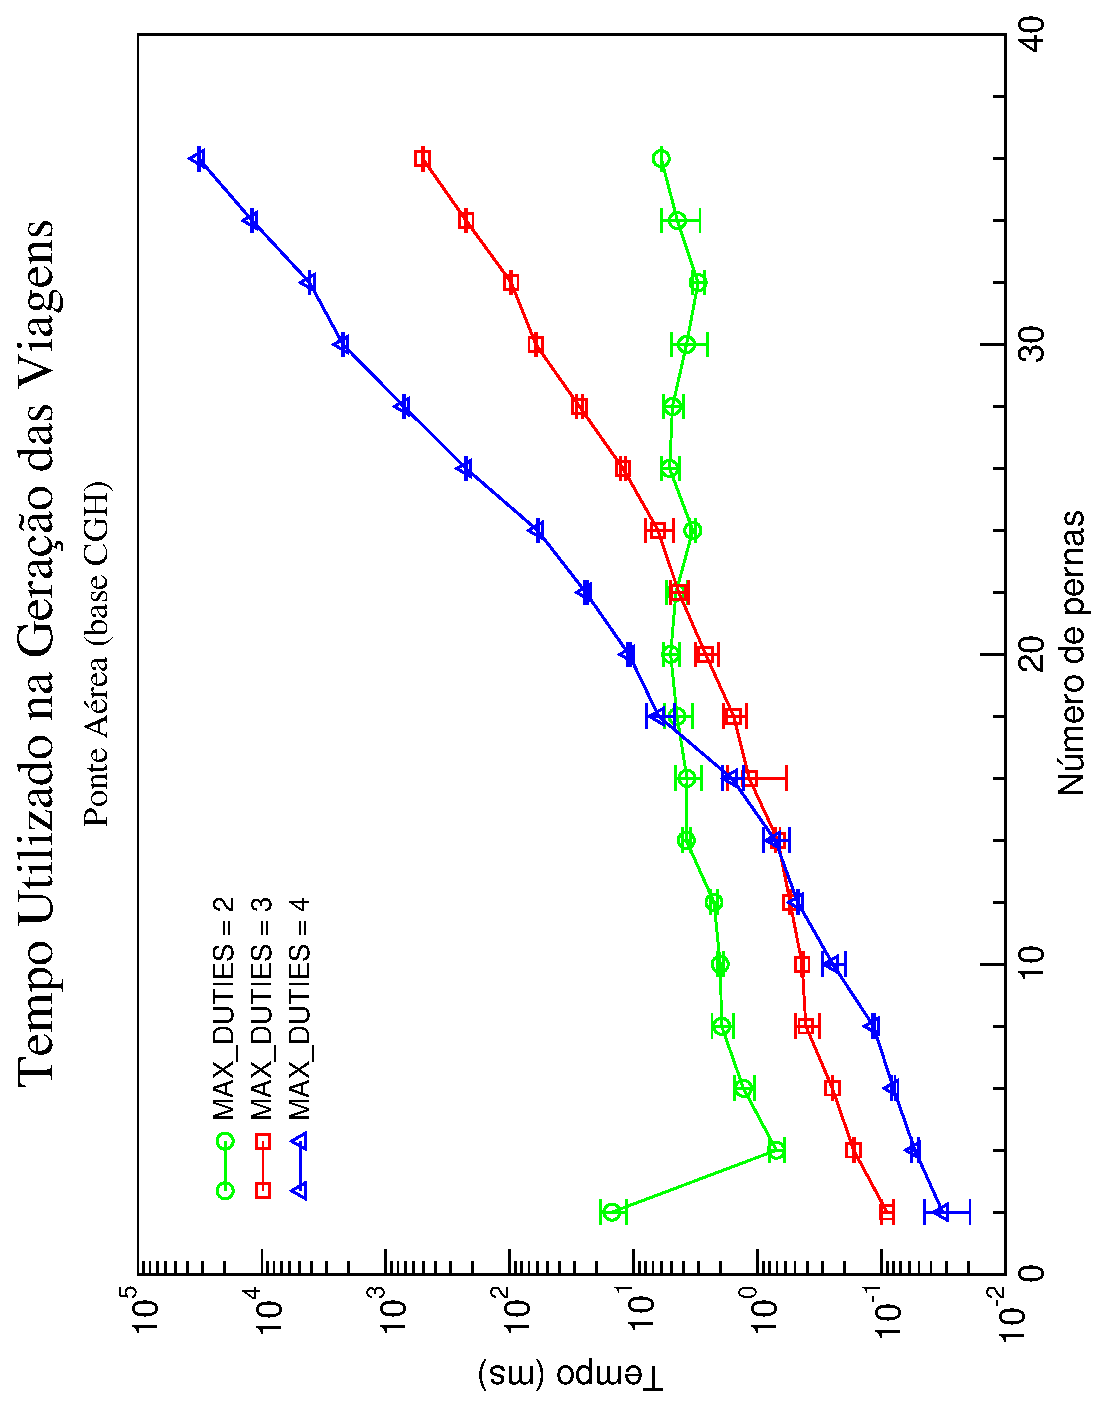
\includegraphics[scale=0.45,angle=-90]{fig/generation_time.eps}
		\caption{Tempo gasto na geração das viagens em função do número de pernas utilizadas na 
		construção da rede de voos. São apresentados valor médio $\pm$ desvio-padrão, considerando 5 
		medidas para cada ponto. O primeiro ponto da curva verde encontra-se um pouco fora provavelmente
		devido a algum transiente da máquina, visto que ele foi o primeiro a ser processado.}
		\label{fig:generation}
	\end{center}
\end{figure}

O tempo gasto pelo otimizador GLPK para resolver o modelo proposto é apresentado no gráfico da 
Figura~\ref{fig:glpk}. Mais uma vez, observa-se um crescimento exponencial muito forte (note a 
escala logarítmica do eixo vertical) em função do número de etapas considerado. A 
Figura~\ref{fig:cplex} mostra os resultados obtidos para o otimizador Cplex. 

\begin{figure}[htb]
	\begin{center}
		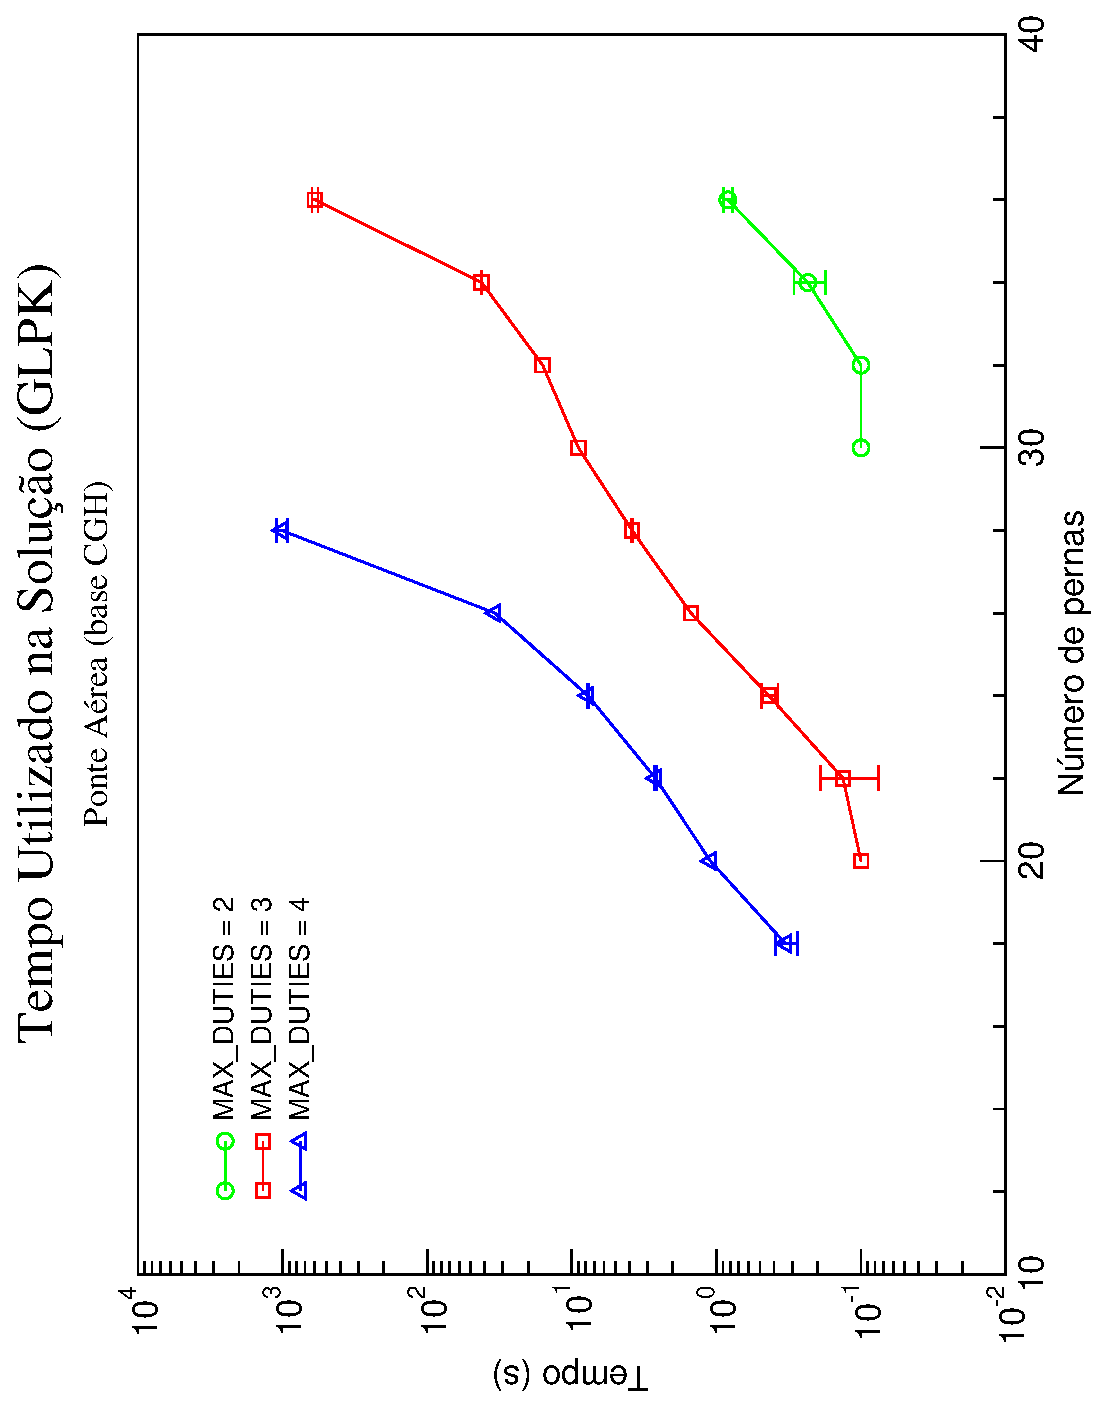
\includegraphics[scale=0.45,angle=-90]{fig/glpk_solution_time.eps}
		\caption{Tempo utilizado pelo otimizador GLPK na obtenção de uma solução inteira, em função do 
		número de etapas. São apresentados valor médio $\pm$ desvio-padrão, considerando 3 medidas para 
		cada ponto. Valores medidos com tempo de execução de 0,0~s não são apresentados (número pequeno 
		de pernas). Os últimos pontos da curva azul não puderam ser estimados, mesmo após algumas horas 
		de processamento.}
		\label{fig:glpk}
	\end{center}
\end{figure}

\begin{figure}[htb]
	\begin{center}
		\includegraphics[scale=0.45,angle=0]{fig/cplex_solution_time.eps}
		\caption{Resultados obtidos para o otimizador Cplex. Valem as mesmas observações feitas na 
		legenda da Figura~\ref{fig:glpk}.}
		\label{fig:cplex}
	\end{center}
\end{figure}

%%%%%%%%%%%%%%%%%%%%%%%%%%%%%%%%%%%%%%%%%%%%%%%%%%%%%%%%%%%%%%%%%%%%%%%%%%%%%%%%%%%%%%%%%%%%%%%%%%%%

\section{Instâncias Estudadas}
\label{sec:instancias}

%%%%%%%%%%%%%%%%%%%%%%%%%%%%%%%%%%%%%%%%%%%%%%%%%%%%%%%%%%%%%%%%%%%%%%%%%%%%%%%%%%%%%%%%%%%%%%%%%%%%

\section{Soluções Exatos}
\label{sec:solucoes_exatas}

Apenas três instâncias (pequenas) puderam ser resolvidas exatamente pela solução do modelo {\it set
partition} (\ref{eq:sppv}), com um tempo de processamento pequeno. A descrição das instâncias é
apresentada na Tabela~\ref{tab:instancias}, as quais foram extraídas de dados reais fornecidos por
companhias aéreas brasileiras. Na tabela são indicados o nome da instância, a companhia a qual
pertence, a frota de aeronaves (ou parte dela) a que se refere, as bases domiciliares dos
tripulantes, o número de etapas e o número de trilhos. O trilho identifica o conjunto de etapas que
uma determinada aeronave da frota deve executar diariamente. No caso de uma frota com $k$ aeronaves,
deverão ser fornecidos $k$ trilhos distintos.

\begin{table}[htb]
	\begin{center} 
		\begin{tabular}{|l|l|l|l|l|l|}
			\hline 
			{\bf Instância} & {\bf Cia} & {\bf Frota} & {\bf Bases} & {\bf Etapas} & {\bf Trilhos} \\ 
			\hline \hline
			73H\_26 & Gol & 737-800 & GRU & 26 & 5 \\ 
			738\_48 & WebJet & 737-800 & GRU GIG & 48 & 7 \\ 
			733\_92 & WebJet & 737-300 & GRU GIG POA & 92 & 12 \\ \hline
		\end{tabular}
		\caption{Caracterização das instâncias resolvidas exatamente através dos modelos 
		{\it set partition} e {\it set cover}. GRU = São Paulo, GIG = Rio de Janeiro e 
		POA = Porto Alegre.}
		\label{tab:instancias}
	\end{center}
\end{table}

Na resolução dos problemas, foram utilizados os parâmetros da Tabela~\ref{tab:parametros}. Além
disso, limitou-se a 1 o número máximo de trocas de aeronaves por jornada. Com isso, forçamos a
tripulação acompanhar, na medida do possível, o trilho percorrido pela aeronave, reduzindo a
possibilidade de conexões em cada localidade. Naturalmente os tempos de conexão serão reduzidos,
tornando as viagens geradas mais baratas e diminuindo o número total de variáveis geradas. Além
disso, esse procedimento torna a solução mais robusta, uma vez que o atraso de uma aeronave não
acarretará atraso na saída de outro voo que dependa daquela aeronave na troca.

O custo de uma viagem foi calculado como sendo o tempo ``ocioso'' relativo no qual o tripulante está 
trabalhando mas não está voando, ou seja, pela diferença entre o tempo total de uma viagem, menos o 
tempo total de voo efetuado, descontando ainda os tempos mínimos regulamentares de conexão entre 
pernas e de descanso entre jornadas, dividido pelo tempo total de voo. Esse custo avalia de forma 
relativa a produtividade de uma viagem, o qual deve ser minimizado na solução final.

Os resultados obtidos são apresentados e resumidos na Tabela~\ref{tab:resultados}. Nela são 
indicadas a instância resolvida, o número total de variáveis geradas, o número de viagens na 
solução, o custo da solução e o tempo de processamento do otimizador (Cplex).

\begin{table}[htb]
	\begin{center} 
		\begin{tabular}{|c|c|c|c|c|}
			\hline 
			{\bf Instância} & {\bf Variáveis} & {\bf Viagens} & {\bf Custo} & {\bf Tempo (s)} \\ 
			\hline \hline
			73H\_26 & 180 & 6 & 6,952 & $< 1$ \\ 
			738\_48 & 66411 & 6 & 6,436 & 3,75 \\
			733\_92 & 1023818 & 11 & 6,942 & 170,86 \\ \hline
		\end{tabular}
		\caption{Resultados obtidos na geração e otimização de viagens para as instâncias consideradas.}
		\label{tab:resultados}
	\end{center}
\end{table}

As mesmas instâncias 73H\_26, 738\_48, 733\_92 também foram resolvidas utilizando o modelo 
{\it set cover}, o qual admite a existência de {\it deadheading}. Os resultados obtidos foram 
idênticos aos listados na Tabela~\ref{tab:resultados}. Em particular, todas as variáveis 
artificiais $y_i$ receberam valor zero na solução final, indicando a não necessidade de 
{\it deadheading}.

%%%%%%%%%%%%%%%%%%%%%%%%%%%%%%%%%%%%%%%%%%%%%%%%%%%%%%%%%%%%%%%%%%%%%%%%%%%%%%%%%%%%%%%%%%%%%%%%%%%%

\section{Um Resultado Explícito}
\label{sec:resultado_explicito}

Para tornar mais concreto a entrada e a saída do problema, apresentamos na Tabela~\ref{tab:73H_26} o
conjunto de etapas referentes a instância 73H\_26\footnote{Não há problema de confidencialidade nos
dados apresentados.}. A mesma representa 26 trechos oferecidos diariamente pela companhia aérea Gol
para uma frota especial de 5 aeronaves B737-800. Para cada etapa são fornecidos o seu número,
aeroporto de origem, aeroporto de destino, horário local de decolagem (DEP) e horário local de pouso
(ARR) e o trilho correspondente.

Na Tabela~\ref{tab:pairings} listamos as 6 viagens geradas como solução do problema de otimização.
Cada etapa na tabela apresenta o número do voo, origem e destino, horário local de decolagem e 
pouso, e o trilho executado. O custo final resultante foi de 6,952, para um total de 180 variáveis 
geradas, considerando a base GRU (São Paulo). Observe a presença de uma viagem bate-volta (4),
bem como uma viagem de 3 dias de duração (5).

\begin{table}[!htb]
	\begin{center}
		\begin{tabular}{|cccccc|}
			\hline 
			{\bf Número} & {\bf Origem} & {\bf Destido} & {\bf DEP} & {\bf ARR} & {\bf Trilho} \\
			\hline \hline
			7625 & GRU &	GIG	 &  07:00	 &  08:00  & 1 \\
			7622 & GIG &	GRU	 &  09:00	 &  09:55	 & 1 \\
			7622 & GRU &	CCS	 &  11:00	 &  15:30	 & 1 \\
			7622 & CCS &	AUA	 &  16:10	 &  17:55	 & 1 \\
			7623 & AUA &	CCS	 &  21:20	 &  22:05	 & 1 \\
			7623 & CCS &	GRU	 &  22:45	 &  06:00	 & 1 \\
			1841 & CWB &	GRU	 &  07:52	 &  08:55	 & 2 \\
			1902 & GRU &	NAT	 &  11:00	 &  14:20	 & 2 \\
			1903 & NAT &	GRU	 &  15:30	 &  19:10	 & 2 \\
			1704 & GRU &	MAO	 &  21:15	 &  00:10	 & 2 \\
			1798 & GRU &	REC	 &  08:05	 &  11:21	 & 3 \\
			1149 & REC &	GRU	 &  12:04	 &  15:30	 & 3 \\
			7680 & GRU &	AEP	 &  18:25	 &  21:15	 & 3 \\
			7681 & AEP &	GRU	 &  22:40	 &  01:30	 & 3 \\
			1705 & MAO &	GRU	 &  03:42	 &  08:35	 & 4 \\
			1766 & GRU &	CWB	 &  09:20	 &  10:16	 & 4 \\
			1846 & CWB &	GRU	 &  11:13	 &  12:15	 & 4 \\
			7480 & GRU &	ASU	 &  13:05	 &  13:50	 & 4 \\
			1847 & GRU &	CWB	 &  18:10	 &  19:20	 & 4 \\
			1767 & CWB &	GRU	 &  20:56	 &  21:50	 & 4 \\
			1566 & GRU &	CWB	 &  22:35	 &  23:30	 & 4 \\
			7481 & ASU &	GRU	 &  14:30	 &  17:25	 & 4 \\
			7678 & GRU &	AEP	 &  08:00	 &  10:50	 & 5 \\
			7679 & AEP &	GRU	 &  11:50	 &  14:35	 & 5 \\
			7658 & GRU &	EZE	 &  15:15	 &  18:15	 & 5 \\
			7659 & EZE &	GRU	 &  20:35	 &  23:25	 & 5 \\ \hline
	\end{tabular}
	\caption{Dados de entrada da instância 73H\_26, contendo 26 etapas e 5 trilhos.}
	\label{tab:73H_26}
	\end{center}
\end{table}

\begin{table}[!htb]
	\begin{center}
		\begin{tabular}{|c|c|ccccc|}
			\hline
			{\bf Viagem} & {\bf Jornada} & \multicolumn{5}{|c|}{\bf Etapa} \\ \hline \hline
			\multirow{6}{*}{1} & \multirow{4}{*}{1}  
			  & 7625 & GRU-GIG & 07:00 & 08:00 & 001 \\
			& & 7622 & GIG-GRU & 09:00 & 09:55 & 001 \\
			& & 7622 & GRU-CCS & 11:00 & 15:30 & 001 \\
			& & 7622 & CCS-AUA & 16:10 & 17:55 & 001 \\ \cline{2-7}
			                       & \multirow{2}{*}{2}
				& 7623 & AUA-CCS & 21:20 & 22:05 & 001 \\
			& &	7623 & CCS-GRU & 22:45 & 06:00 & 001 \\ \hline \hline
			\multirow{2}{*}{2} & \multirow{2}{*}{1}  		
				& 1902 & GRU-NAT & 11:00 & 14:20 & 002 \\
			& & 1903 & NAT-GRU & 15:30 & 19:10 & 002 \\ \hline \hline
			\multirow{2}{*}{3} & \multirow{1}{*}{1}  		
				& 1704 & GRU-MAO & 21:15 & 00:10 & 002 \\ \cline{2-7}
                           	& \multirow{1}{*}{2}
				&	1705 & MAO-GRU & 03:42 & 08:35 & 004 \\ \hline \hline
			\multirow{2}{*}{4} & \multirow{2}{*}{1}  		
				& 1798 & GRU-REC & 08:05 & 11:21 & 003 \\
			& & 1149 & REC-GRU & 12:04 & 15:30 & 003 \\ \hline \hline			
			\multirow{10}{*}{5} & \multirow{3}{*}{1}  
				&	1847 & GRU-CWB & 18:10 & 19:20 & 004 \\
			& &	1767 & CWB-GRU & 20:56 & 21:50 & 004 \\
			& &	1566 & GRU-CWB & 22:35 & 23:30 & 004 \\ \cline{2-7}
                           		& \multirow{4}{*}{2}
				&	1841 & CWB-GRU & 07:52 & 08:55 & 002 \\
			&	&	1766 & GRU-CWB & 09:20 & 10:16 & 004 \\
			&	&	1846 & CWB-GRU & 11:13 & 12:15 & 004 \\
			&	&	7480 & GRU-ASU & 13:05 & 13:50 & 004 \\ \cline{2-7}
                           		& \multirow{3}{*}{3}
				&	7481 & ASU-GRU & 14:30 & 17:25 & 004 \\
			&	&	7680 & GRU-AEP & 18:25 & 21:15 & 003 \\
			&	&	7681 & AEP-GRU & 22:40 & 01:30 & 003 \\ \hline \hline
			\multirow{4}{*}{6} & \multirow{3}{*}{1}  
				& 7678 & GRU-AEP & 08:00 & 10:50 & 005 \\
			& & 7679 & AEP-GRU & 11:50 & 14:35 & 005 \\
			&	& 7658 & GRU-EZE & 15:15 & 18:15 & 005 \\ \cline{2-7}
                           	 & \multirow{1}{*}{2}
				& 7659 & EZE-GRU & 20:35 & 23:25 & 005 \\ \hline
		\end{tabular}
		\caption{Conjunto de viagens obtido como solução ótima da instância 73H\_26.}
		\label{tab:pairings}
	\end{center}
\end{table}

%%%%%%%%%%%%%%%%%%%%%%%%%%%%%%%%%%%%%%%%%%%%%%%%%%%%%%%%%%%%%%%%%%%%%%%%%%%%%%%%%%%%%%%%%%%%%%%%%%%%
			                               
\section{Busca Local}
\label{sec:resultados_busca}

%%%%%%%%%%%%%%%%%%%%%%%%%%%%%%%%%%%%%%%%%%%%%%%%%%%%%%%%%%%%%%%%%%%%%%%%%%%%%%%%%%%%%%%%%%%%%%%%%%%%

\section{Algoritmo Genético}
\label{sec:resultados_genetico}

%%%%%%%%%%%%%%%%%%%%%%%%%%%%%%%%%%%%%%%%%%%%%%%%%%%%%%%%%%%%%%%%%%%%%%%%%%%%%%%%%%%%%%%%%%%%%%%%%%%%

\section{Geração de Colunas}
\label{sec:resultados_cg}

%%%%%%%%%%%%%%%%%%%%%%%%%%%%%%%%%%%%%%%%%%%%%%%%%%%%%%%%%%%%%%%%%%%%%%%%%%%%%%%%%%%%%%%%%%%%%%%%%%%%

\section{Implementações}
\label{sec:implementacoes}

%%%%%%%%%%%%%%%%%%%%%%%%%%%%%%%%%%%%%%%%%%%%%%%%%%%%%%%%%%%%%%%%%%%%%%%%%%%%%%%%%%%%%%%%%%%%%%%%%%%%

\zerar
\chapter{Conclusão}
\label{cap:conclusoes}

Com relação a análise preliminar apresentada na Seção~\ref{sec:analise_p}, concluímos que o
procedimento de geração de viagens leva a um número gigantesco de variáveis, mesmo para um pequeno
número de pernas (Figura~\ref{fig:pairings}). Isso porque a natureza combinatória do problema leva o
algoritmo de busca a explorar diversas possibilidades, principalmente em uma rede como a da ponte
aérea, onde existem diversas possibilidades de conexão toda vez que se chega em uma das localidades.
Além disso, essas possibilidades se multiplicam quando consideramos um maior número de jornadas
permitidas (\verb|MAX_DUTIES|). Apesar disso, a geração de viagens ainda se fez em tempo aceitável,
podendo ser aplicada para redes maiores (Figura~\ref{fig:generation}).

Entretanto, quando esse número enorme de variáveis é levado ao otimizador, o tempo de processamento
se torna impraticável. Para se certificar disso, basta extrapolar as curvas obtidas nas
Figuras~\ref{fig:glpk} e~\ref{fig:cplex}. {\bf Uma tentativa de resolução de uma instância da
ponte-aérea contendo 40 etapas, não pode ser resolvida mesmo após 12 horas de processamento.} Ainda
assim, ficamos surpresos com a capacidade do otimizador resolver instâncias com um número de
variáveis da ordem de $10^6$ em tempo aceitável (resultados da Tabela~\ref{tab:resultados}).

A análise preliminar então nos mostra que o método de ``gerar-e-otimizar'' para resolver o modelo
(\ref{eq:sppv}) não é adequado para resolver o problema de forma geral. Em particular, das milhares
de variáveis geradas, apenas poucas delas são escolhidas para entrar na solução final, como se pode
observar da Tabela~\ref{tab:resultados}. Isso indica que o procedimento de geração explícita de 
variáveis não é adequado, pois muitas delas não servem para nada. Um procedimento mais inteligente
seria o de gerar apenas variáveis ``boas'', ou seja, com grande chance de aparecerem na solução 
final. O método de geração de colunas desenvolve essa ideia e será explorado futuramente.

Com relação aos resultados obtidos utilizando o modelo {\it set cover}, observamos que como as 
colunas associadas às variáveis $y_i$ de {\it deadheading} (reveja o formulação (\ref{eq:scpdv})) 
foram ajustadas com preços altos, e como os problemas analisados eram viáveis do ponto de vista do 
{\it set partition}, o otimizador conseguiu encontrar as mesmas soluções obitidas sem a presença de 
{\it deadheading}. Concluímos que a utilização de {\it deadheading} só será realizada se for 
estritamente necessária para viabilidade do problema.

%%%%%%%%%%%%%%%%%%%%%%%%%%%%%%%%%%%%%%%%%%%%%%%%%%%%%%%%%%%%%%%%%%%%%%%%%%%%%%%%%%%%%%%%%%%%%%%%%%%%

\section{Comparação Entre Heurísticas}
\label{sec:comparacao}

%%%%%%%%%%%%%%%%%%%%%%%%%%%%%%%%%%%%%%%%%%%%%%%%%%%%%%%%%%%%%%%%%%%%%%%%%%%%%%%%%%%%%%%%%%%%%%%%%%%%

\section{Perspectivas Futuras}
\label{sec:perspectivas}




\part{Subjetivo}

\chapter{Análise Subjetiva}
\label{cap:analise_subjetiva}

\section{Daniel Augusto Cortez}
\label{sec:daniel_subjetiva}

\newpage
\section{Lucas Rodrigues Colucci}
\label{sec:lucas_subjetiva}

Até meu irmão ingressar no curso de Bacharelado em Ciências da Computação no IME, os programas de
computador funcionavam, na minha visão, através de mágica. Após seu ingresso, percebi que não era
magia e sim um monte de letras e números que, até então, não faziam sentido. Decidi que não
cometeria o mesmo ``erro'' e, caso não passasse na sonhada Engenharia Mecânica da POLI, faria um ano
de cursinho.

Não passei na POLI e fiquei em uma posição na qual não teria chances de ingresso em nenhuma das
quatro chamadas. Comecei o cursinho e, logo no primeiro dia, fiquei entediado com a rotina de
estudos. No terceiro dia um amigo me informou que eu havia passado na quarta chamada do BCC, e,
devido à insatisfação com o cursinho, comecei a pensar no assunto.

Pesquisei sobre a carreira de cientistas da computação e notei a possibilidade de uma boa
remuneração, e, em algumas empresas, de um estilo de trabalho descontraído. Optei por enfrentar o
desafio e ingressar no curso. Imaginava que, caso não gostasse do curso, poderia pedir transferência
para a POLI.

\subsection{IME/BCC}

Ao longo desses quatro anos, pensei diversas vezes em desistir do curso devido à sua dificuldade. No
entanto, após cursar as disciplinas de física, meu sonho de cursar engenharia já não existia mais e
decidi concluir a faculdade.

Com o tempo, fui pegando gosto pela programação e, aliado ao envolvimento com a atlética e com o
time de basquete, a vida no IME tornou-se mais fácil e agradável.


\subsection{Disciplinas}

Ao longo do curso, me deparei com disciplinas em que não entendia o por que de serem ministradas
para o BCC. No entanto, hoje vejo que todas foram de suma importância para minha formação, seja na
construção do raciocínio lógico ou na teoria da programação.

A seguir cito as matérias que considero mais importantes para a minha formação:

\begin{itemize} 
	\item Introdução à Computação: ensina e desmistifica o que é a programação;
	\item Princípios de Desenvolvimento de Algoritmos: promove a aprendizagem de alguns dos tópicos
mais importantes da computação como ordenação e lista ligada; 
	\item Análise de Algoritmos: apesar de ser uma matéria mais matemática, após a disciplina damos mais ênfase à eficiência do software durante seu desenvolvimento;
	\item Algoritmos em Grafos: essencial para resolver muitos problemas reais, inclusive o problema        de geração de viagens de nosso trabalho;
	\item Programação Linear: matéria mais interessante do curso. Ensina a arte da otimização, assunto de grande interesse para a maioria das empresas;
	\item Laboratório de Programação I e II e Engenharia de Software: primeiras oportunidades de trabalhar em programas extensos e em grupo; 
	\item Laboratório de Programação Extrema: disciplina na qual simulamos o trabalho em uma empresa
de software, com clientes e cobranças. Essencial para aprendermos como agir em diversas situações e
aperfeiçoar relações interpessoais;
\end{itemize}

\subsection{Projeto do TCC}

Logo no começo do curso, devido à necessidade de tirar dúvidas com outros alunos, comecei a me
relacionar com dois alunos do BCC: Daniel e Renato. A partir daí estudávamos e fazíamos trabalhos
sempre juntos.

No começo deste ano, após nos matricularmos na disciplina do TCC, começamos a pensar em um projeto
no qual pudéssemos trabalhar juntos. Após algumas idéias descartadas, o Daniel nos apresentou a
oportunidade de fazer um projeto muito interessante relacionado ao seu trabalho. Fomos
comentar a idéia com nosso orientador, o professor Alfredo, e ele aprovou a idéia.

Fizemos muitas pesquisas, lemos muitos papers sobre o assunto e começamos a implementação. Após
muito trabalho, terminamos o TCC e tivemos ótimos resultados. Isso fez todos os quatro anos de
graduação valerem a pena, mostrando que estamos preparados para enfrentar os mais difíceis desafios.

\subsection{Comentários Finais}

O que mais senti falta durante a minha formação foi do incentivo, por parte dos professores, de
realizarmos trabalhos em grupo. O mundo profissional exige uma boa relação entre pessoas, e isso não
é praticado no IME. Apesar disso, percebo que muitas das dificuldades geradas pelo curso foram
essenciais para meu amadurecimento e capacidade de enfrentar desafios.

Gostaria de deixar aqui meus agradecimentos aos coautores desse projeto, Daniel e Renato, os quais
me ajudaram ao longo de toda a graduação e se tornaram grandes amigos. Agradeço também aos meus
pais, Miguel e Angela, que sempre me incentivaram a continuar no curso; ao meu irmão, Thiago, que,
além de me incentivar, me ajudou em muitas das matérias; ao nosso orientador, Alfredo, que se
mostrou um grande professor e nos ajudou em todos os problemas do projeto; e à minha namorada e
melhor amiga, Aline, que mostrou-me que todos temos dificuldades e que o segredo da felicidade está
em como nos comportamos perante a elas.

\newpage
\section{Renato Lerac Corrêa de Sá}
\label{sec:renato_subjetiva}

O mundo da informática sempre fez parte da minha vida. Na época de garoto, jogos eletrônicos eram o
meu passatempo predileto e, ao ganhar meu primeiro computador, minha curiosidade sobre como tudo
funcionava despertou. Pesquisando por conta própria, aprendi sobre os diversos componentes que
constituem uma máquina moderna e a relação entre eles. A partir deste ponto, comecei a montar meus
próprios computadores, peça por peça, sempre buscando as últimas inovações tecnológicas.

Devido ao meu interesse por hardware, ingressei na Escola Politécnica da USP com o objetivo de
cursar Engenharia da Computação. Foi então que tive o primeiro contato com programação e desde então
meu interesse por softwares apenas aumentou.

Aliando meu novo interesse ao grande crescimento pelo qual a área de tecnologia da informação
vem passando nos últimos anos e a falta de profissionais qualificados no mercado, optei por
abandonar o curso de engenharia e ingressar no curso de Bacharelado em Ciências da Computação do
IME.

\subsection{IME/BCC}

Estou prestes a me formar e agora consigo enxergar o curso de uma forma mais abrangente. Sinto que o
instituto forneceu-me uma excelente base teórica, de modo que hoje possuo conhecimento sobre as mais
diversas áreas relacionadas à tecnologia da informação. Acredito que este deveria ser o objetivo de
qualquer curso de graduação, isto é, proporcionar ao graduando um aprendizado amplo sobre sua área,
de forma que ele tenha conhecimento suficiente para escolher uma especialização ao fim do curso, se
desejar.

\subsection{Disciplinas}

A grande maioria das disciplinas cursadas foi essencial à minha formação e, direta ou
indiretamente, importante no desenvolvimento deste trabalho. Faço, no entanto, uma lista
com as disciplinas que considero mais importantes. Primeiramente, gostaria de citar as disciplinas
que fundamentam a base do curso:

\begin{itemize}
	\item Cálculo Diferencial e Integral e Álgebra: quase todas as áreas do curso requerem algum
	conhecimento matemático. Estas disciplinas dão a base necessária para que o graduando
	sinta-se confortável ao lidar com matemática;
	\item Estatística e Processos Estocásticos: probabilidades e distribuições estão presentes
	em diversas disciplinas e conhecimento em estatística é fundamental para qualquer
profissional qualificado;
	\item Introdução à Computação: é a disciplina que ensina o graduando a raciocinar através
	de algoritmos, sendo, portanto, a porta de entrada do curso.
\end{itemize}

Algumas disciplinas foram importantes devido ao conhecimento conceitual proporcionado. Entre elas,
destaco:

\begin{itemize}
	\item Princípios de Desenvolvimento de Algoritmos: introduz diversos conceitos necessários
	para a programação, entre eles: recursividade, lista ligada, busca binária e ordenação.
	Promove uma primeira abordagem sobre a eficiência de algoritmos;
	\item Estrutura de Dados: discute métodos eficientes para abstrair entidades e dados reais,
	o que é parte fundamental de qualquer projeto de computação;
	\item Análise de Algoritmos: através de uma abordagem mais intensa sobre a eficiência dos
	algoritmos, introduz conceitos importantes como recorrências, programação dinâmica e
	algoritmos gulosos;
	\item Algoritmos em Grafos: é uma das disciplinas mais interessantes e úteis do curso, já
	que grafos estão presentes em diversos problemas reais;
	\item Programação Linear: apesar de ser o pesadelo de muitos alunos, o conhecimento
	adquirido na disciplina foi importante durante a realização deste trabalho de formatura;
	\item Programação Concorrente: devido à tecnologia multi-core existente hoje, torna-se
	necessário aprender conceitos de concorrência.
\end{itemize}

Um aspecto importante do curso é a prática de programação. Muitas disciplinas exigem
exercícios-programas, mas algumas se destacam por oferecerem experiências únicas ao graduando:

\begin{itemize}
	\item Laboratório de Programação I e II: porporcionam ao aluno as primeiras oportunidades
	para trabalhar em equipe e dedicar-se a projetos mais complexos do que os
	exercícios-programas habituais;
	\item Engenharia de Software: permite ao aluno aplicar conceitos de métodos ágeis em um
	projeto de programação web;
	\item Laboratório de Programação Extrema: é a melhor disciplina do curso. O aluno trabalha
	em projetos reais com sua equipe, respondendo diretamente a um cliente. Tudo feito em um
	ambiente descontraído;
	\item Trabalho de Formatura Supervisionado: foi muito bom ter como última experiência no
	curso a chance de unir todo o conhecimento adquirido em 4 anos de luta em um extenso projeto
	de pesquisa e desenvolvimento. Além disso, foi interessante conhecer os trabalhos dos
	colegas	de curso.
\end{itemize}

Por fim, devido ao meu grande interesse por hardware, gostaria de mencionar duas disciplinas que,
embora não sejam fundamentais para a formação, foram de grande valor:

\begin{itemize}
	\item Sistema Operacionais: por desvendar a mágica por trás dos sistemas operacionais
	modernos e esclarecer como é realizada a comunicação entre software e hardware;
	\item Organização de Computadores: por mergulhar no mundo do hardware e apresentar 
	diferentes arquiteturas.
\end{itemize} 

\subsection{Projeto do TCC}

Durante estes 4 anos de curso, desenvolvi uma amizade muito grande com os co-autores deste trabalho:
Daniel e Lucas. Em todas as disciplinas que cursamos juntos, sempre realizamos trabalhos e estudos
em equipe. Foi natural que decidíssimos desenvolver o TCC juntos, apesar da maior cobrança a que um
trabalho em equipe está sujeito.

Como o Daniel é comandante em uma companhia aérea, decidimos que seria interessante fazer um
trabalho relacionado. Nosso orientador Alfredo pediu desde o início que realizássemos um projeto
considerando a realidade brasileira. O Daniel então sugeriu o problema da otimização de viagens e
nosso orientador ficou logo entusiasmado.

Foram necessárias várias semanas de pesquisa para que obtivéssemos o conhecimento necessário sobre o
problema. Todavia, quanto mais pesquisávamos o assunto, maior se tornava o interesse da equipe.
Então, junto com nosso orientador Alfredo, optamos por bater o martelo, na certeza de que o projeto
seria muito trabalhoso, mas que no fim valeria a pena.

Gostaria de agredecer o Professor Alfredo, cuja ajuda durante estes longos meses de pesquisa e
desenvolvimento foi importantíssima. Acho que cumprimos nossos objetivos e espero que possamos
escrever o artigo sugerido pelo Professor.

\subsection{Comentários Finais}

Apesar da qualidade da formação, acho que é importante ressaltar alguns pontos negativos. Em
primeiro lugar, a cobrança é excessiva em alguns casos. A maioria das disciplinas demanda uma
enorme quantidade de horas dedicadas fora dos horários de aula. Isto é um problema ainda maior para
quem trabalha ou por algum outro motivo não possui tanto tempo livre para se dedicar aos estudos.

Em segundo lugar, é complicado cobrar o conteúdo de algumas disciplinas em provas escritas. A
necessidade de provas em tais disciplinas poderia ser revista. Como exemplo, posso citar Engenharia
de Software e Laboratório de Programação.

Por último, acredito que o trabalho em equipe pode ser mais estimulado ao longo do curso. É
importante realizar programação pareada nos EPs, mas são poucas as disciplinas em que
realmente podemos trabalhar em equipe.

Enfim, vale dizer que foi necessária muita dedicação para chegar ao final do curso. Os professores
são excelentes profissionais e sempre estiveram dispostos a ajudar. Saio do IME com uma base de
conhecimento sólida e abrangente, que me permitirá realizar trabalhos em diferentes áreas.




\bibliography{../bib/crew_scheduling}
\bibliographystyle{plain}

\end{document}

